\section{Results}
\label{sec:results}

\subsection{AIMSpice}

The register could have different effect and operations due to the corner of the transistor and the temperature. There are five corners the transistors could be; TT(typical-typical), SS(slow-slow), FF(fast-fast), SF(slow-fast) and FS(fast-slow).  For all of the corners they have been tested for three temperatures, 0$^\circ C$, 27$^\circ C$ and 70$^\circ C$. All the different plots for the different cases are shown in the appendix \ref{appendix:aimspicePlots}. 

To validate the functionality of the register, one can examine the plot of the TT and FF corner at 27$^\circ C$. 

\begin{figure}[H]
    \centering
    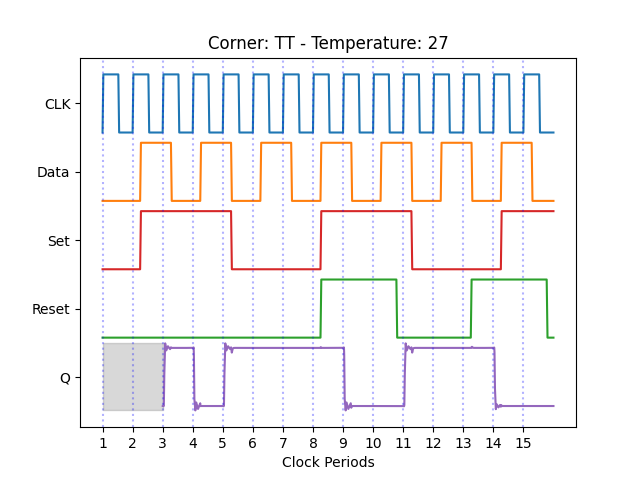
\includegraphics[width=\textwidth]{Figures/Aimspice_Plots/TT_27.png}
    \caption{Plot of register for TT corner}
    \label{fig:result_TT27}
\end{figure}

As shown in figure \ref{fig:result_TT27} and figure \ref{fig:result_FF27}, the different combinations of the inputs signals. If set is high, Q only updates to the D-value when the CLK changes from low to high. And if the reset is high, the value Q is overruled to low, even if set and D is high.

When looking at the different corners and temperatures, the difference of the functionality is quite similar. One can see in this case with the TT and FF corners at 27$^\circ C$, that the register is just a tiny fraction more stable with a FF corner rather than a TT corner.

\begin{figure}[H]
    \centering
    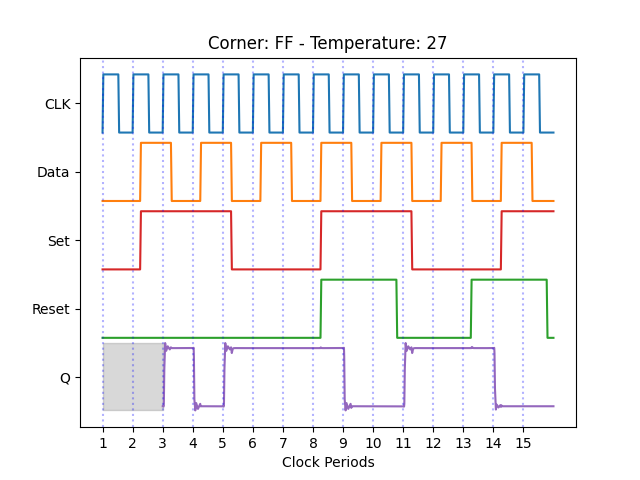
\includegraphics[width=\textwidth]{Figures/Aimspice_Plots/FF_27.png}
    \caption{Plot of register for FF corner}
    \label{fig:result_FF27}
\end{figure}

\subsubsection{Static Power Consumption}

As explained in section \ref{subsec:low_power}, a low voltage on $V_{DD}$ is optimal. We have therefore chosen a value for $V_{DD} = 0.85V$, as a lower $V_{DD}$ gives a lower power consumption. By using the function operating point in AIMSpice, the leakage current in the $V_{DD}$ node can be found.

Table \ref{tab:leakage} shows the different leakage current for the TT and FF corners with all three temperatures. To calculate the static power consumption, we use the formula \ref{eq:power} for all the values and get table \ref{tab:power}.

\begin{table}[H]
\centering
\caption{Leakage Current}
\label{tab:leakage}
\resizebox{0.4\columnwidth}{!}{%
    \begin{tabular}{lll}
    \cline{2-3}
    \multicolumn{1}{l|}{} &
      \multicolumn{1}{l|}{TT} &
      \multicolumn{1}{l|}{FF} \\ \hline
    \multicolumn{1}{|l|}{0 $^\circ$C} &
      \multicolumn{1}{l|}{1.0931 nA} &
      \multicolumn{1}{l|}{3.1854 nA} \\ \hline
    \multicolumn{1}{|l|}{27 $^\circ$C} &
      \multicolumn{1}{l|}{3.0325 nA} &
      \multicolumn{1}{l|}{8.5711 nA} \\ \hline
    \multicolumn{1}{|l|}{70 $^\circ$C} &
      \multicolumn{1}{l|}{6.9843 nA} &
      \multicolumn{1}{l|}{13.513 nA} \\ \hline
     &  &  
    \end{tabular}%
}
\end{table}

\begin{table}[H]
\centering
\caption{Static Power Consumption}
\label{tab:power}
\resizebox{0.4\columnwidth}{!}{%
\begin{tabular}{lll}
\cline{2-3}
\multicolumn{1}{l|}{} &
  \multicolumn{1}{l|}{TT} &
  \multicolumn{1}{l|}{FF} \\ \hline
\multicolumn{1}{|l|}{0 $^\circ$C} &
  \multicolumn{1}{l|}{0.92914 nW} &
  \multicolumn{1}{l|}{2.7076 nW} \\ \hline
\multicolumn{1}{|l|}{27 $^\circ$C} &
  \multicolumn{1}{l|}{2.5776 nW} &
  \multicolumn{1}{l|}{7.2854 nW} \\ \hline
\multicolumn{1}{|l|}{70 $^\circ$C} &
  \multicolumn{1}{l|}{5.9367 nW} &
  \multicolumn{1}{l|}{11.486 nW} \\ \hline
 &  &  
\end{tabular}
}
\end{table}

\subsection{Verilog}

In this subsection results of Verilog-simulation will be presented. All Verilog-code is given in \autoref{appendix:Verilog-code}.

\autoref{fig:fsm_simulation} shows the FSM simulated for randomized inputs $I_1$ and $I_0$.

\begin{figure}[H]
    \centering
    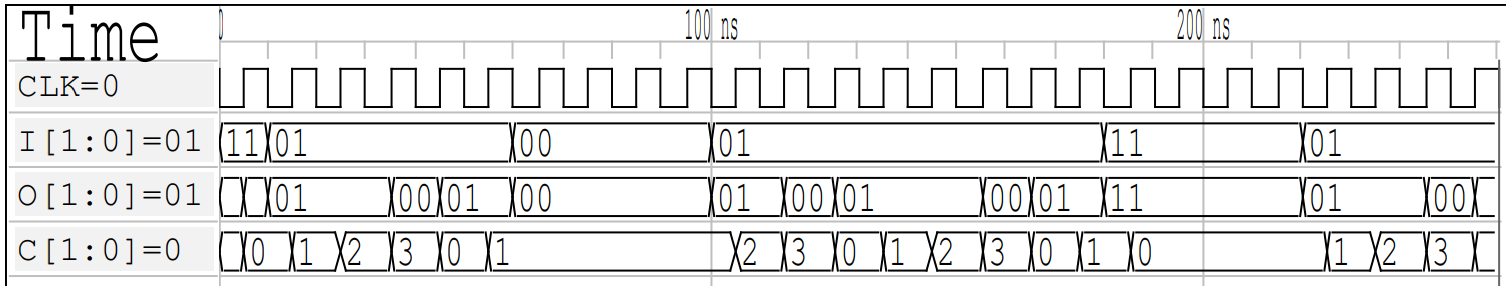
\includegraphics[width=\textwidth]{Figures/FSM_testbench_out.png}
    \caption{Timing diagram of FSM simulated in Verilog}
    \label{fig:fsm_simulation}
\end{figure}

From the figure we see that the memory transitions to the expected states based on the inputs. The FSM begins in state ''Run-1'' and transitions to state ''Reset'' as the reset input $I_1$ is set high. The next state is ''Run-1'', then ''Run-2''. The Run-bit $I_0$ is then set low, resulting in a two-period pause in state ''Pause-2''. Further the FSM transitions to ''Run-3'', ''Pause'' and ''Run-1''.

This simulation was run and verified to follow the wanted behaviour as given by table x.

\autoref{fig:eightbitadder_sim} shows a simulation of the 8-bit adder with random 8-bit inputs A and B. Note that all values in the timing diagram are hexadecimal and that any overflow-bits are handled outside our system. The code used for this simulation is given in \autoref{verilog_eightbitadder}.

\begin{figure}[H]
    \centering
    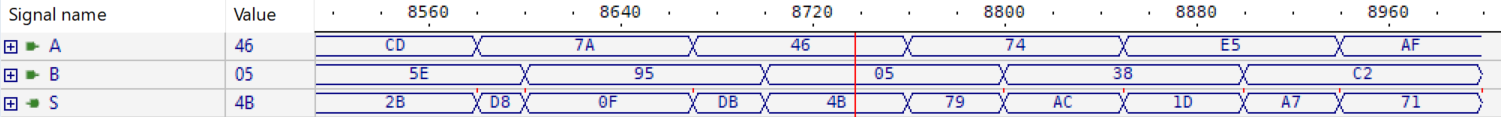
\includegraphics[width=\textwidth]{Figures/Test of eightbitadder.png}
    \caption{Timing diagram of 8-bit adder simulated in Verilog}
    \label{fig:eightbitadder_sim}
\end{figure}

\autoref{fig:dflipflop_sim} shows a simulation of a single D Flip-Flop realized in Verilog.

\begin{figure}[H]
    \centering
    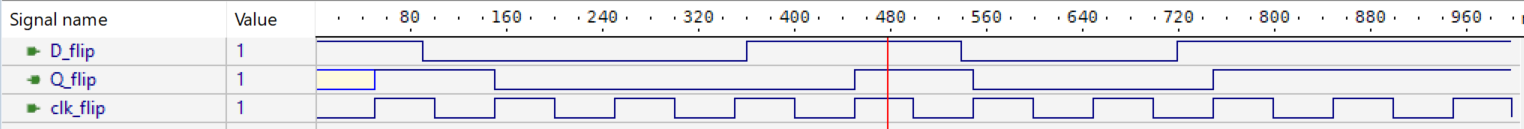
\includegraphics[width=\textwidth]{Figures/Test of Dflipflop.png}
    \caption{Timing diagram of D Flip-Flop simulated in Verilog}
    \label{fig:dflipflop_sim}
\end{figure}

\autoref{fig:8bitregister_sim} shows a simulation of a 8-bit register realized in Verilog.

\begin{figure}[H]
    \centering
    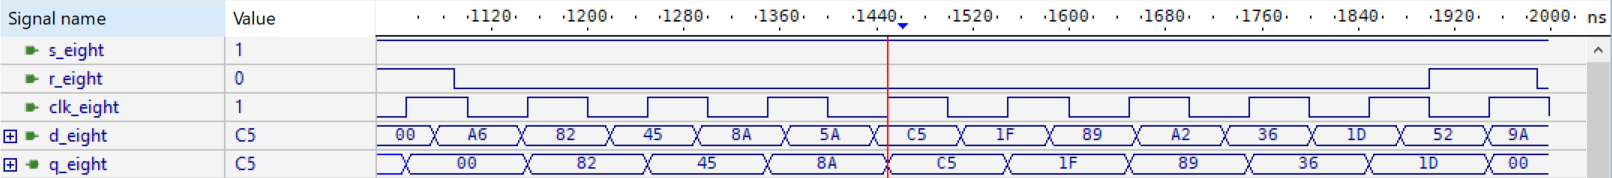
\includegraphics[width=\textwidth]{Figures/VerilogPlot_8bitreg.png}
    \caption{Timing diagram of an 8-bit register simulated in Verilog}
    \label{fig:8bitregister_sim}
\end{figure}

\autoref{fig:multiplier_sim} shows a simulation of the 2-bit multiplier realized in Verilog. Inputs A and B are stimulated with arbitrary two bit values to observe the possible outputs. The multiplier has a 4-bit output as the largest possible output result, 9, needs four bits to be represented in binary.

\begin{figure}[H]
    \centering
    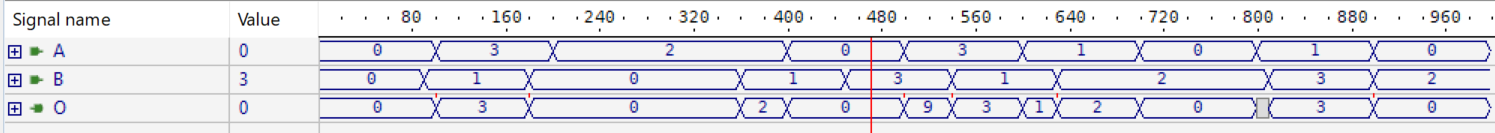
\includegraphics[width=\textwidth]{Figures/Test of multiplier.png}
    \caption{Timing diagram of multiplier simulated in Verilog}
    \label{fig:multiplier_sim}
\end{figure}



% Present the results of your simulations in this section. Use tables and graphs or other figures to illustrate your results. Remember: The table caption goes above the table, the figure caption goes below the figure.

% The results section must include:
% \begin{itemize}
%     \item Figures and/or tables that show the results of your simulation.
%     \item Text that describe what we see in the simulation results (e.g. as expected we can see that XYZ which means the circuit functions as intended).
%     \item NB! The result section is a \textit{what?}-section. \textit{What} where the results? \textit{What} do the figures/results mean? Any \textit{why}-questions you might want to write about and try to answer typically belong in the discussion section.
% \end{itemize}